\documentclass[11pt]{article}

\usepackage[utf8]{inputenc}  %francais et caractères
\usepackage[T1]{fontenc} 
\usepackage[francais]{babel}
\usepackage{lscape}

\usepackage{amsmath} %math

\usepackage{graphicx} %images
\usepackage{wrapfig} %images dans texte

\usepackage[dvipsnames]{xcolor} %couleurs
\usepackage{appendix} %annexes
\usepackage{listings} %insertion de lignes de code
\usepackage{physics}
\usepackage{mathtools, stmaryrd}
%\usepackage[framed,numbered,autolinebreaks,useliterate]{mcode}

\newenvironment{rmq}[1] {\noindent\HRule\par\vspace{5pt}\textbf{\textit{REMARQUE : }}#1}{\\\HRule\par\vspace{5pt}}

\renewcommand\lstlistingname{Code}
\renewcommand{\lstlistlistingname}{Table de Codes}

\lstset{language=VHDL,%
    %basicstyle=\color{red},
    breaklines=true,%
    keywordstyle=\color{Orange},
    identifierstyle=\color{Cyan},
    stringstyle=\color{Red},
    commentstyle=\color{Green},
    morekeywords={matlab2tikz},
    morekeywords=[2]{1}, keywordstyle=[2]{\color{white}},
    showstringspaces=false,%without this there will be a symbol in the places where there is a space
    numbers=left,%
    numberstyle={\tiny \color{black}},% size of the numbers
    numbersep=9pt, % this defines how far the numbers are from the text
    emph=[1]{for,end,break},emphstyle=[1]\color{red}, %some words to emphasise
    %emph=[2]{word1,word2}, emphstyle=[2]{style}, 
    backgroundcolor=\color{Black},
    basicstyle=\scriptsize\color{White}\ttfamily,
    frame=L,
    captionpos = b,
    %===========================================================
    framesep=3pt,%expand outward.
    framerule=0.4pt,%expand outward.
    xleftmargin=3.4pt,%make the frame fits in the text area. 
    xrightmargin=3.4pt,%make the frame fits in the text area.
    %=========================================================== 
    rulecolor=\color{Red}   
}


\usepackage[right=2cm, left=2cm, top=2cm, bottom=2cm]{geometry}

\newcommand{\HRule}{\rule{\linewidth}{0.5mm}}

\begin{document}

% Page de Garde
\noindent 
DURAND Clovis \\ MAGNAN Camille\hfill{12 Mai 2017}
% // et entrer d'autres noms. 



\vspace{2cm}
\begin{center}
    \Large{PG208} %Inserer la matiere concernée
    \HRule \\[0.1cm]
    {\textsc{\LARGE \textbf{PG208 \\ Dessin vectoriel}}}\\
    \HRule\\[02cm]
    \Large{V1}
\end{center}
\vspace{1,5cm}

\begin{figure}[htbp]
    \begin{center}
        
\includegraphics[width=10cm]{Logo-quadri.png}
    \end{center}
\end{figure}

\vspace{1cm}
\begin{center}
    \Large{ENSEIRB-Matmeca \\ Bordeaux - Talence}
\end{center}

\vspace{2cm}
%Encadrant : Machin

\newpage
% Tables
\tableofcontents
%\lstlistoflistings
\listoffigures
\newpage 

% Debut doc

\section{Introduction}

L'objectif de ce projet est de mettre en œuvre les notions de base de la programmation orientée objets appliquées au langage C++ que l'on a appréhendées durant l’enseignement de PG208. Pour ce faire nous avons décidé de nous lancer dans le second sujet de projet: \textbf{Dessin vectoriel}. L'objectif est de générer une image Bitmap en fonction d'un fichier de description vectoriel de formes. L'enjeu de ce sujet est de comprendre l’intérêt de l'utilisation de classes et d'apprendre à faire interagir les différentes classes entre elles. \\

Cette application est appelé \texttt{dessin\_vect}

\subsection{Gestion du cahier des charges}

Nous avons donc tenté de réaliser une application permettant de suivre au mieux le cahier des charges qui nous a été soumis. En effet, nous avons développé un programme permettant de générer des images à l’aide d’une description vectorielle de ces images. Ces images seront créées à partir de la descriptions de plusieurs formes géométriques. Nous avons donc programmé le dessin de 10 formes différentes afin d'avoir un large panel de possibilités graphiques : la ligne, le triangle vide, le point, le cercle (vide et plein), le rectangle (vide et plein) et enfin le carré (vide et plein). 

Le cahier des charges stipule que nous devons gérer un facteur d'échelle qui modifie la résolution de notre image de sortie. Un facteur de transparence doit aussi être intégré lorsqu'on dessine une forme. 

Voici le diagramme de cas d'utilisation qui représente le mode d'opération du point de vue du client : 

\begin{figure}[!htbp]
    \begin{center}
        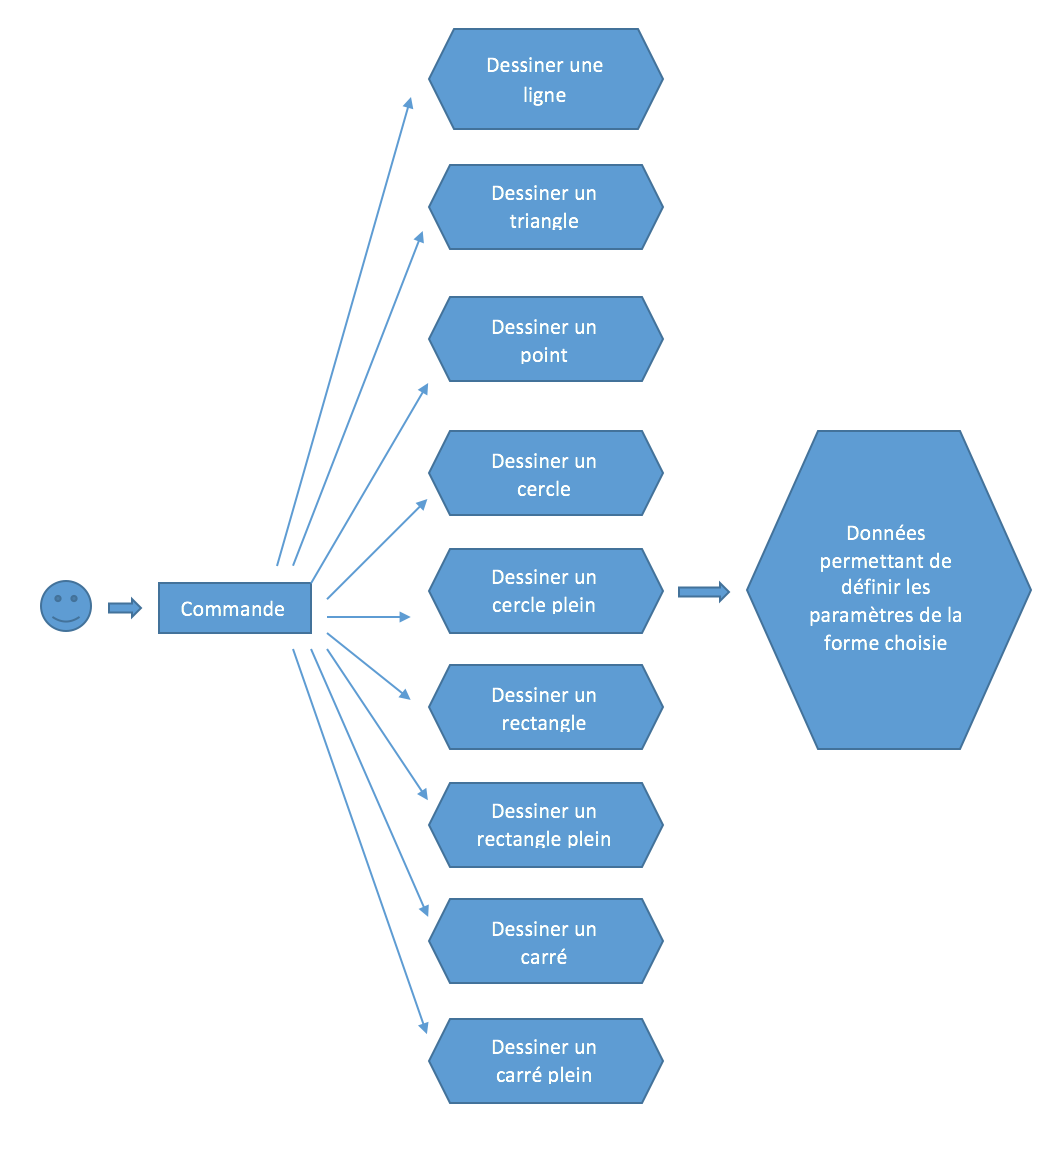
\includegraphics[width=13cm]{Photo1.png}
        \caption[Diagramme des cas d'utilisation]{Diagramme de cas d'utilisation de notre programme \texttt{dessin\_vect}}
    \centering
    \end{center}
\end{figure}

\clearpage

\subsection{Diagramme UML}

Le langage UML est un langage de modélisation graphique à base de pictogrammes conçu pour fournir une méthode simple pour visualiser la conception d'un système. Nous avons donc utilisé ce langage afin de nous de nous permettre de suivre un cheminement clair et détaillé de notre projet. Ce diagramme permet aussi de comprendre comment les différentes classes ont été construites les unes par rapport aux autres, comme les rapports d'héritage. \\

\begin{figure}[!htbp]
    \begin{center}
        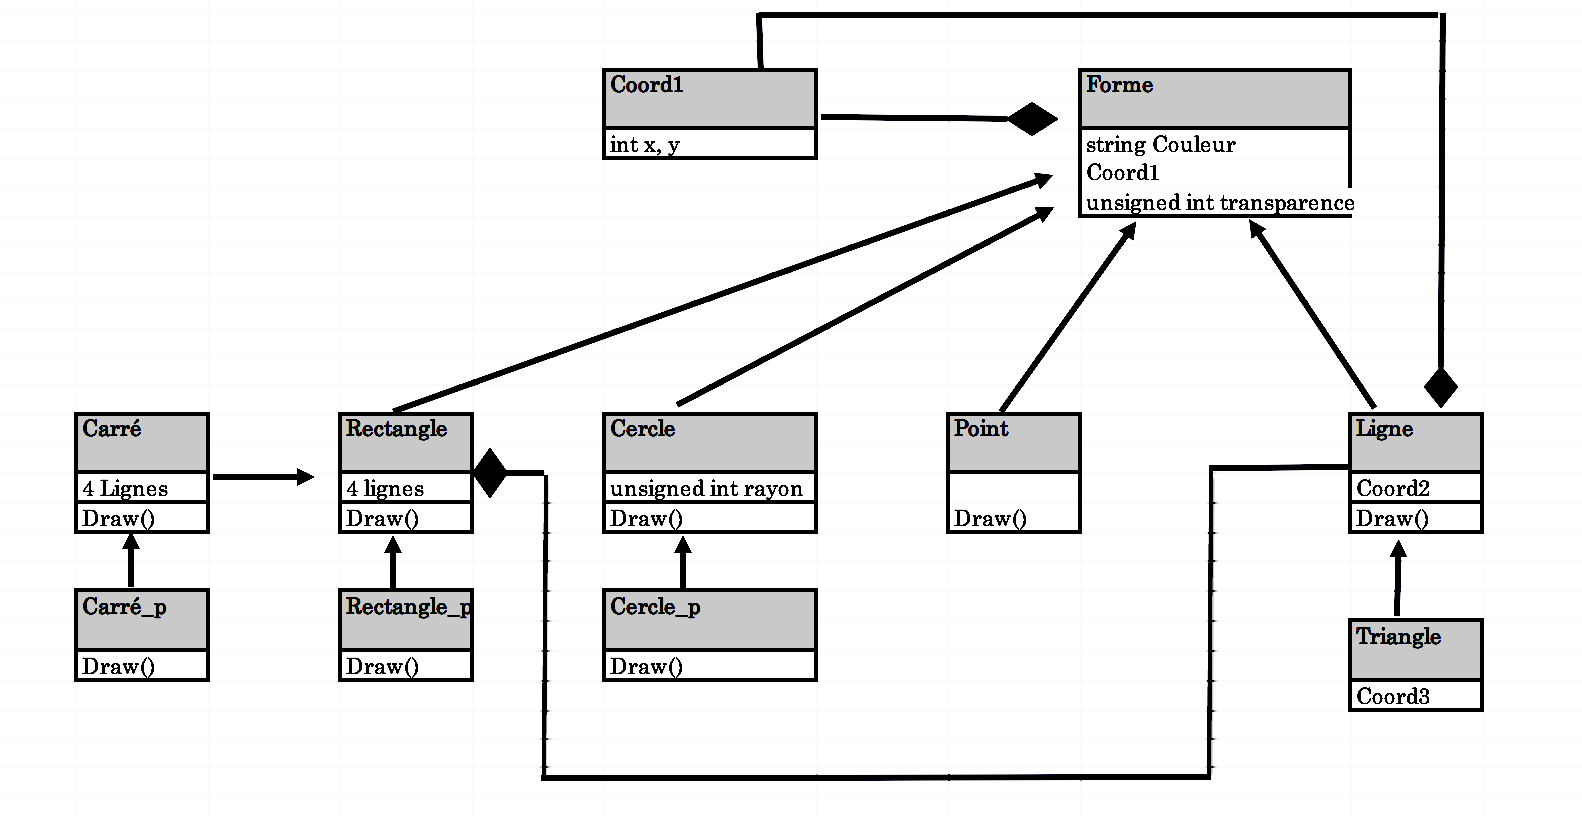
\includegraphics[width=20cm]{Photo2.png}
        \caption{diagramme UML}
    \centering
    \end{center}
\end{figure}

\section{Les classes principales}

Grâce au diagramme UML vu précédemment, nous avons pu commencer à écrire le code de notre projet par les classes principales. En effet certaines des classes à programmer sont plus importantes que les autres. Nous avons fait le choix de créer une classe de coordonnées Coord (non indispensable mais qui nous a permis de nous approprier la notion de position d'un objet dans l'image dès le début) qui rassemble les coordonnées x et y de chaque forme. \\

Nous avons commencé par concevoir la classe forme contient tous les attributs communs aux futures classes des différentes formes. 

Ensuite, nous avons écrit le reste des classes de formes, en commençant par la classe Ligne. Celle-ci est à la base de beaucoup de formes. Par exemple, la méthode \texttt{drawLigne()} est utilisée dans toutes les formes (mis à part la classe Cercle et la classe Cercle\_p).

Enfin une classe Dessin permet de réunir toutes les formes en un seul objet, de définir les bornes de l'image, et de fournir les informations au dessin de l'image. 

\subsection{Classe de coordonnées Coord}

La classe \texttt{Coord} est une classe pratique. Celle-ci ne génère pas une forme, mais permet simplement de généraliser les 2 coordonnées d'un point en un seul objet. Cet objet servira d'attribut pour la classe Forme, ainsi que pour d'autres formes. 

\subsection{Classe forme \texttt{Forme}}

La classe mère Forme regroupe l'ensemble des attributs communs à toutes les classes de formes :

\\

\begin{itemize}
    \item Coord m\_c1 : Cette coordonnée définit la position dans l'image de l'objet. Ce point sert de base pour construire le reste de la forme. 
    \item string m\_couleur : La couleur de l'objet. Tous les objets à dessiner doivent avoir une couleur définie, de manière à écrire cette couleur sur un pixel de l'image. Pour ce faire un format RGB est utilisé (0 à 255 pour chacune des trois couleur primordiales). 
    \item unsigned int m\_transparence : Ce facteur permet de définir le niveau de transparence de la forme sur le dessin. 
\end{itemize}

Elle regroupe également les méthodes utilisées dans les différentes formes, c'est à dire la méthode générant la couleur des pixels en fonction des valeurs de R, G et B. De cette façon il nous est possible de récupérer la valeur de R, G et B indépendamment afin de déterminer la couleur de notre pixel. Nous avons rajouté une fonction \texttt{DrawPixel} dans la classe CImage qui nous permet de dessiner chaque pixel grâce à un simple appel à cette fonction. Cette classe nous permet également de déterminer le réglage de couleur du pixel en fonction du niveau de transparence retenu grâce à la formule suivante : 

\begin{figure}[!htbp]
    \begin{center}
        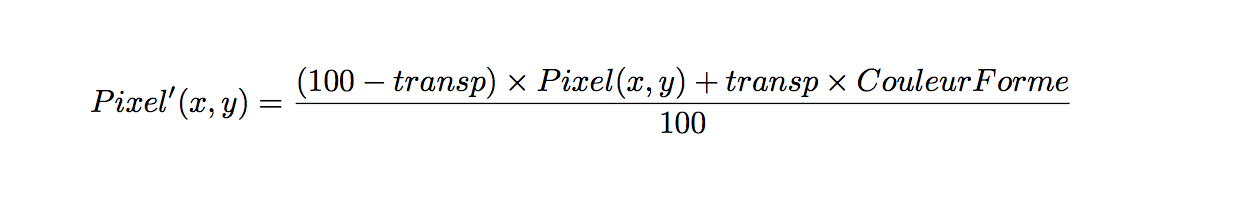
\includegraphics[width=12cm]{Formule.png}
    \centering
    \end{center}
\end{figure}


\subsection{Classe Dessin \texttt{Dessin}}

A REMPLIRRRE

\clearpage

\subsection{Classe Ligne \texttt{Ligne}}

Nous avons décidé de tracer nos lignes à l'aide de la méthode de Bresenham. Cette méthode permet d’identifier le sens du tracé de la ligne et de déterminer les pixels que l'on doit dessiner afin de s'approcher le plus près possible d'une ligne droite (avec un taux d'erreurs le plus faible possible). Pour celà, nous séparons l'écran en octants. Nous partons d'un point central, puis nous prenons le deuxième point de la ligne et nous calculons les deltas de la droite reliant ces deux points. Grâce à ceux-ci nous determinons dans quel octant nous nous trouvons et appliquons ainsi l'algorithme de Bresenham dans cet octant. 

\
\

\begin{figure}[!htbp]
    \begin{center}
        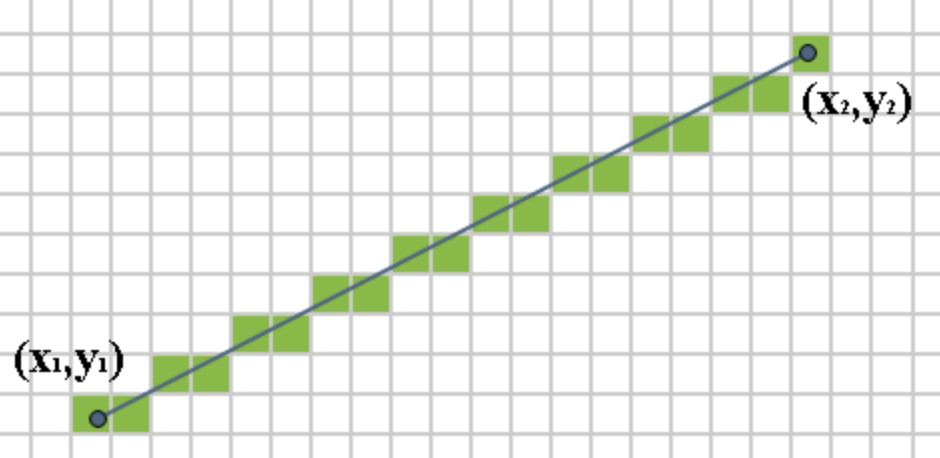
\includegraphics[width=13cm]{Photo3.png}
        \caption{Schéma explicatif de la méthode de Nreenham}
    \centering
    \end{center}
\end{figure}

\clearpage
\section{Classes filles \texttt{Formes diverses}}

\subsection{Le Point \texttt{Point}}

\subsection{Le Cercle \texttt{Cercle \& Cercle\_p}}

\subsubsection{Cercle vide}

De son côté le cercle est défini de la façon suivante : CERCLE (C, RAYON, COULEUR, TRANSPARENCE). Nous utilisons ensuite une condition de longueur, telle que si l'on se trouve à une distance \texttt{RAYON} du centre, alors le pixel est dessiné. Afin d'avoir un tracé suffisement large à l'oeil humain, nous avons ajouté un "epsilon" de sorte que le pixel soit dessiné si il se trouve dans l'intervale \texttt{RAYON +- EPSILON}

\subsubsection{Cercle plein}

Le cercle plein est dessiné d'une façon similaire, sauf que la condition ne porte pas sur un intervale mais seulement sur une infériorité. En effet, on dessine le pixel si il est à une distance inferieure à celle du rayon du centre du cercle.

\subsection{Le Rectangle \texttt{Rectangle \& Rectangle\_p}}

\subsubsection{Rectangle vide}

Le rectangle vide est tout simplement créé à partir de 4 lignes. Ces lignes trouvent leurs coordonnées en fonction du point de départ (coin en bas à gauche du rectangle) et des longueurs et hauteurs.

\subsubsection{Rectangle plein}

Le rectangle plein fonctionne à partir de lignes également. En effet, le remplissage se fait en balayant le rectangle dans la hauteur et en dessinant une ligne à chaque incrémentation.

\subsection{Le Carré \texttt{Carre \& Carre\_p}}


\subsection{Le Triangle \texttt{Triangle}}

Tout comme le rectangle vide, le triangle est créé à partir de 3 lignes.


\subsection{ Aboutissement }


\section{Dimensions graphiques}

JE COMPRENDS RIEN

\end{document}